%-------------------------------------------------------------------------------------------------%
% Author: John Joseph Valletta
% Date: 26/02/2015
% Title: Classification
%-------------------------------------------------------------------------------------------------%
% Preamble
\documentclass[pdf]{beamer}
\usepackage{textpos} % for logo placement in headline
\usepackage[export]{adjustbox}
\usepackage{framed}
%-------------------------------------------------------------------------------------------------%
\usepackage{listings} % To insert code
\usepackage{color}
\definecolor{dkgreen}{rgb}{0,0.6,0}
\definecolor{gray}{rgb}{0.5,0.5,0.5}
\definecolor{mauve}{rgb}{0.58,0,0.82}
\definecolor{deepblue}{rgb}{0,0,0.5}
\definecolor{deepred}{rgb}{0.6,0,0}
\definecolor{deepgreen}{rgb}{0,0.5,0}
\definecolor{lightgray}{rgb}{0.90,0.90,0.90}
\lstdefinestyle{RCode}{
language=R,                     % the language of the code
basicstyle=\scriptsize\ttfamily,       % the size of the fonts that are used for the code
numbers=none,%left,                   % where to put the line-numbers
numberstyle=\tiny\color{gray},  % the style that is used for the line-numbers
stepnumber=1,                   % the step between two line-numbers. If it's 1, each line
                          % will be numbered
numbersep=5pt,                  % how far the line-numbers are from the code
backgroundcolor=\color{lightgray},  % choose the background color. You must add \usepackage{color}
showspaces=false,               % show spaces adding particular underscores
showstringspaces=false,         % underline spaces within strings
showtabs=false,                 % show tabs within strings adding particular underscores
frame=lines,%single,                   % adds a frame around the code
rulecolor=\color{black},        % if not set, the frame-color may be changed on line-breaks within not-black text (e.g. commens (green here))
tabsize=2,                      % sets default tabsize to 2 spaces
captionpos=b,                   % sets the caption-position to bottom
breaklines=true,                % sets automatic line breaking
breakatwhitespace=false,        % sets if automatic breaks should only happen at whitespace
title=\lstname,                 % show the filename of files included with \lstinputlisting;
                          % also try caption instead of title
keywordstyle=\color{blue},      % keyword style
commentstyle=\color{dkgreen},   % comment style
stringstyle=\color{mauve},      % string literal style
escapeinside={\%*}{*)},         % if you want to add a comment within your code
morekeywords={}            % if you want to add more keywords to the set
}
%-------------------------------------------------------------------------------------------------%
\newif\ifplacelogo % Create a new conditional to avoid displaying logo on every slide
\placelogotrue % Set it to true
\mode<presentation>{\usetheme{Madrid}} % default Antibes Berlin Madrid Montpelier Ilmenau CambridgeUS Berkeley Singapore Copenhagen Malmoe Warsaw
\usecolortheme{dolphin}
\useinnertheme{circles} % circles, rectanges, rounded, inmargin
\usefonttheme[onlymath]{serif} % Makes math fonts like the usual LaTeX ones
%\useoutertheme{tree} % infolines, smoothbars, sidebar, split, tree
\setbeamercovered{transparent=5} % Transparent 10% overlays
\setbeamertemplate{caption}{\raggedright\insertcaption\par} % Remove the word "Figure" from caption %\setbeamertemplate{caption}[default]
\setbeamertemplate{navigation symbols}{} % don't put navigation tools at the bottom (alternatively \beamertemplatenavigationsymbolsempty)
\graphicspath{ {./Figures/} }

% Titlepage
\title{Classification}
\subtitle{(supervised learning)}
\author{JJ Valletta}
% \logo{
%   \makebox[0.95\paperwidth]{
%     
\includegraphics[width=4cm,keepaspectratio]{logo1.pdf}
%     \hfill
%     
\includegraphics[width=4cm,keepaspectratio]{logo2.pdf}
%   }
% }
% Logo
\logo{\ifplacelogo
\includegraphics[width=4cm,keepaspectratio, left]{logo2.pdf}\fi}
\addtobeamertemplate{headline}{}{\ifplacelogo
\begin{textblock*}{100mm}(.68\textwidth,+0.1cm)%.015 instead of 0.68 originally

\includegraphics[width=4cm,keepaspectratio]{logo1.pdf}
\end{textblock*}\fi}
%\author{John Joseph Valletta, Alex Thornton and Mario Recker}
%-------------------------------------------------------------------------------------------------%
% Start of Document
%-------------------------------------------------------------------------------------------------%
\begin{document}
%-------------------------------------------------------------------------------------------------%
% Slide 0: Title Slide
\begin{frame}
\titlepage
\end{frame}
\placelogofalse % Turn logo off
%-------------------------------------------------------------------------------------------------%
\begin{frame}{Overview}
\begin{itemize}\addtolength{\itemsep}{0.5\baselineskip}
	\item<2-> The classification task
	\item<3-> Over/under-fitting a predictive model
 	\item<4-> $k$-nearest neighbour ($k$NN)
	\item<5-> Decision trees
	\item<6-> Random forests
	\item<7-> Support vector machines (SVM)
\end{itemize}
\end{frame}
%-------------------------------------------------------------------------------------------------%
\begin{frame}{Classification}
\begin{block}{Definition}
Assigning a set of new observations to a predefined category/class, using a predictive model trained
on observations whose category/class is known
\end{block}
\vfill
\begin{center}
	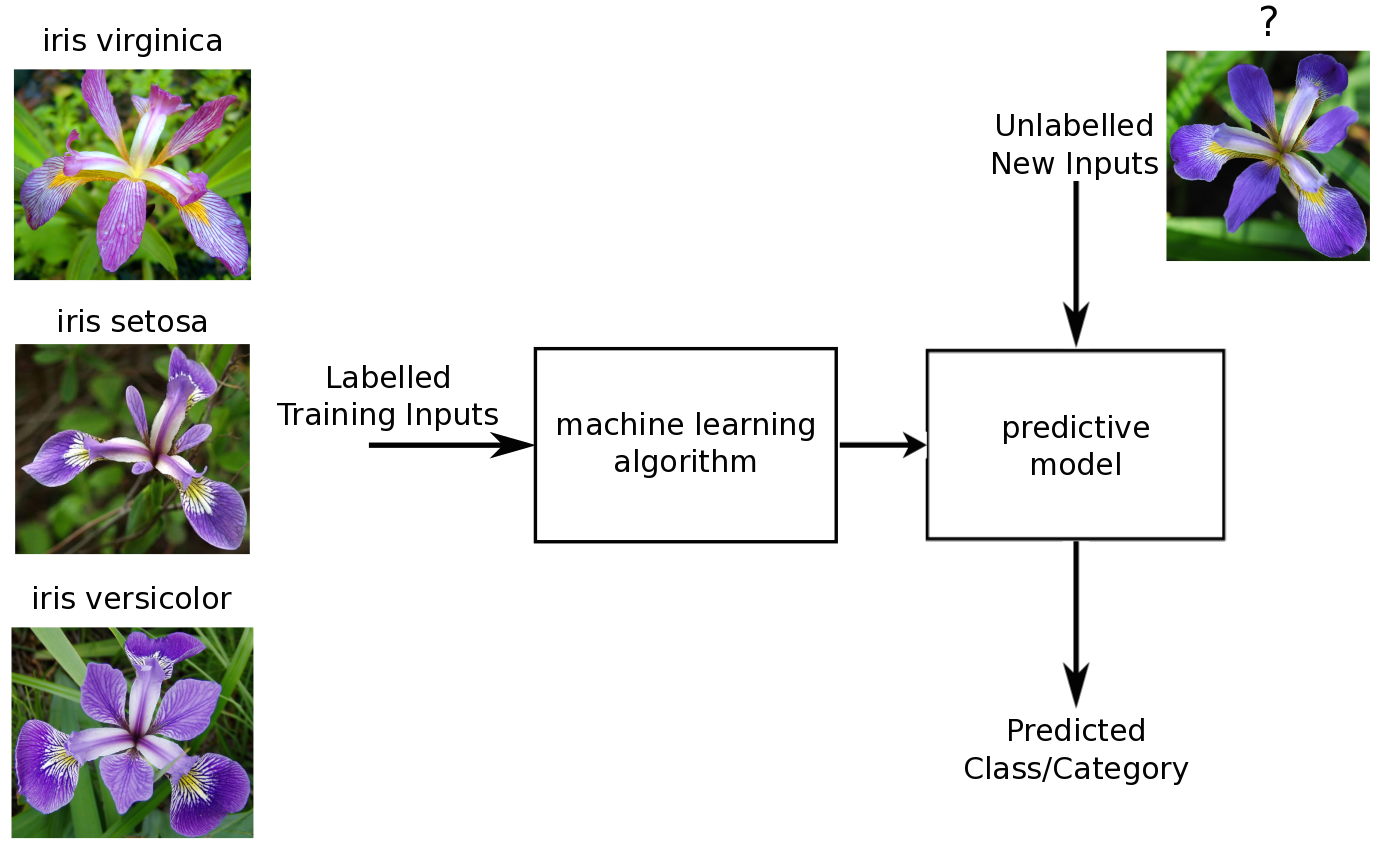
\includegraphics[width=0.72\textwidth]{classification.png}
\end{center}
\vfill
\textbf{Note}: Better data/features will almost always beat better algorithms
\end{frame}
%-------------------------------------------------------------------------------------------------%
\begin{frame}{Where are classifiers used?}
\begin{description}[Biometric authentication:]\addtolength{\itemsep}{0.5\baselineskip}
	\item [Medical imaging:] is tumour benign or cancerous
	\item [Gene expression:] use ``signature'' to classify patient as having (or not) a condition
	\item [Computer vision:] detect and track a moving object
	\item [Biogeography:] classify land cover using remote sensing imagery
	\item [Speech recognition:] translate audio signals into written text
	\item [Biometric authentication:] identify a person using some personal characteristic e.g fingerprint or DNA 
	\item [Epidemiology:] given a set of risk factors what is the chance of patient suffering from a certain condition
\end{description}
\end{frame}
%-------------------------------------------------------------------------------------------------%
\begin{frame}{Over/under-fitting (bias-–variance tradeoff)}
\begin{itemize}\addtolength{\itemsep}{0.5\baselineskip}
\item How well should we fit the training data to get good generalisation?
\item Driving training error to zero is not a good idea
\item \textbf{Bias} caused by a too rigid model leads to \textit{underfitting}
\item \textbf{Variance} caused by a too flexible model leads to \textit{overfitting}
\item \textbf{Occam's Razor}, pick the simplest model that explains your data, \textit{parsimony}
\end{itemize}
\begin{center}
	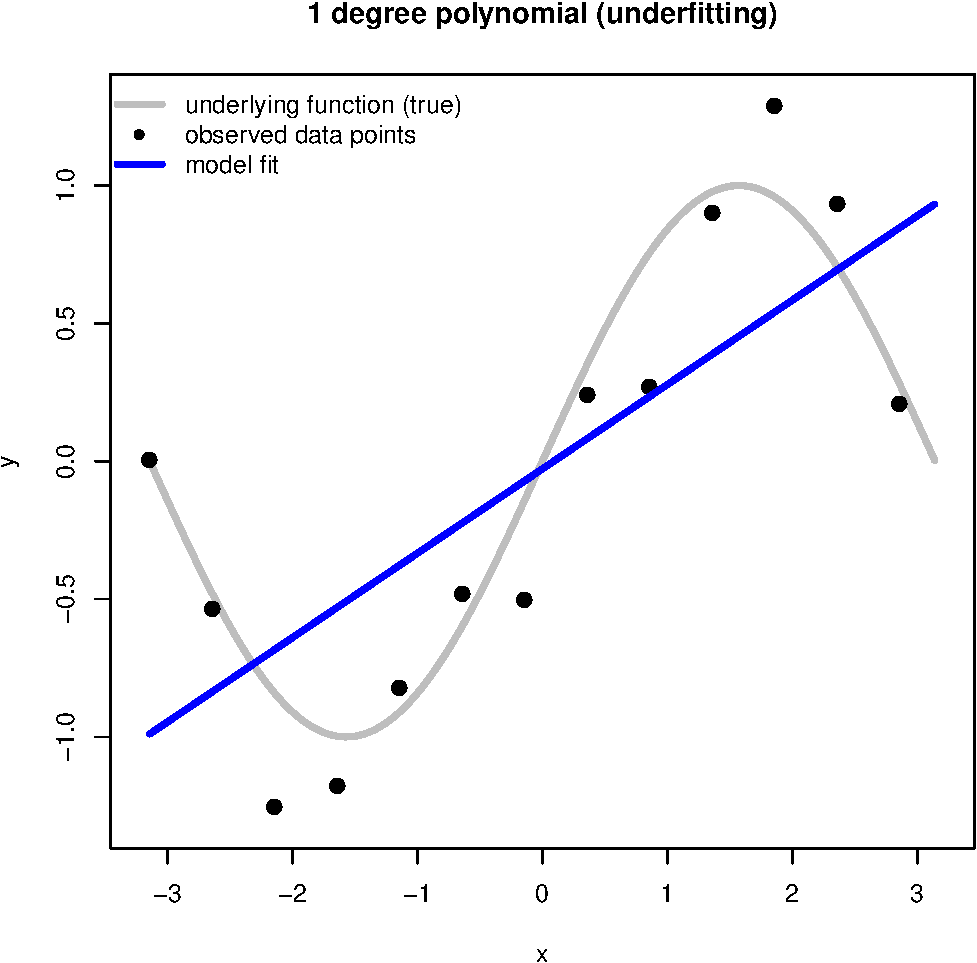
\includegraphics[width=0.333\textwidth]{polyFit1.pdf}
	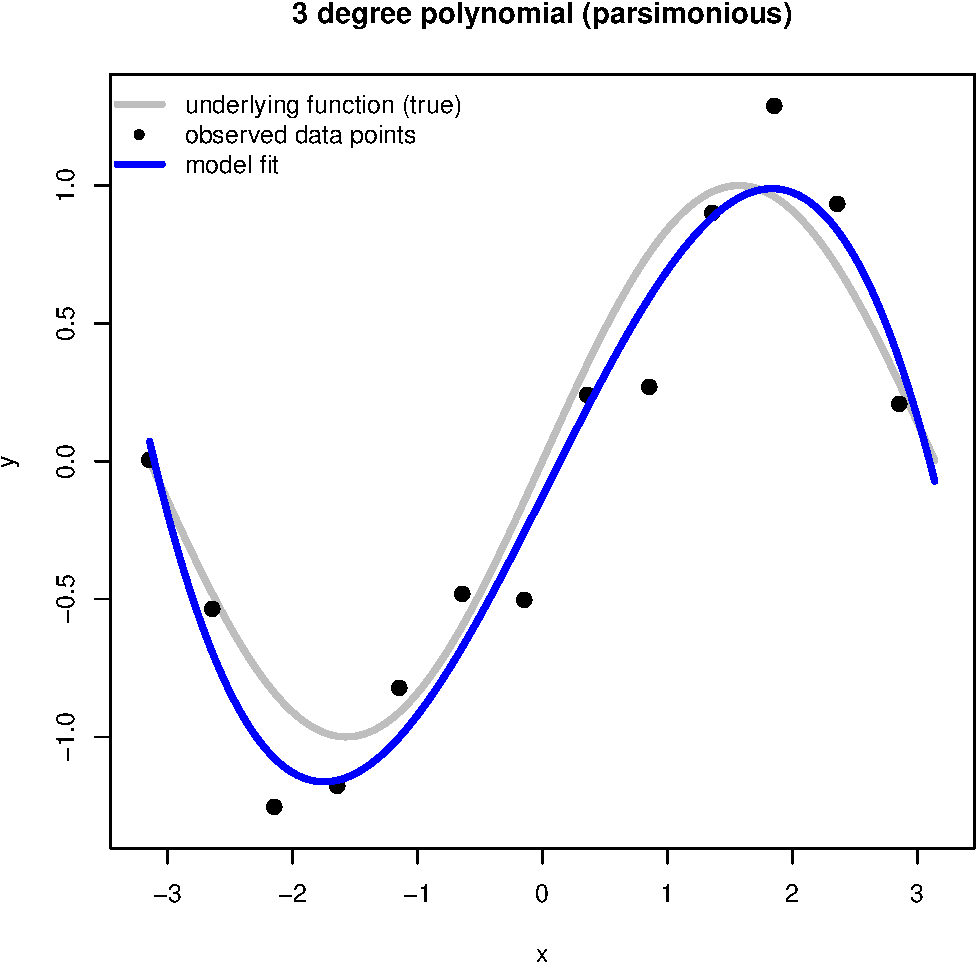
\includegraphics[width=0.333\textwidth]{polyFit3.pdf}
	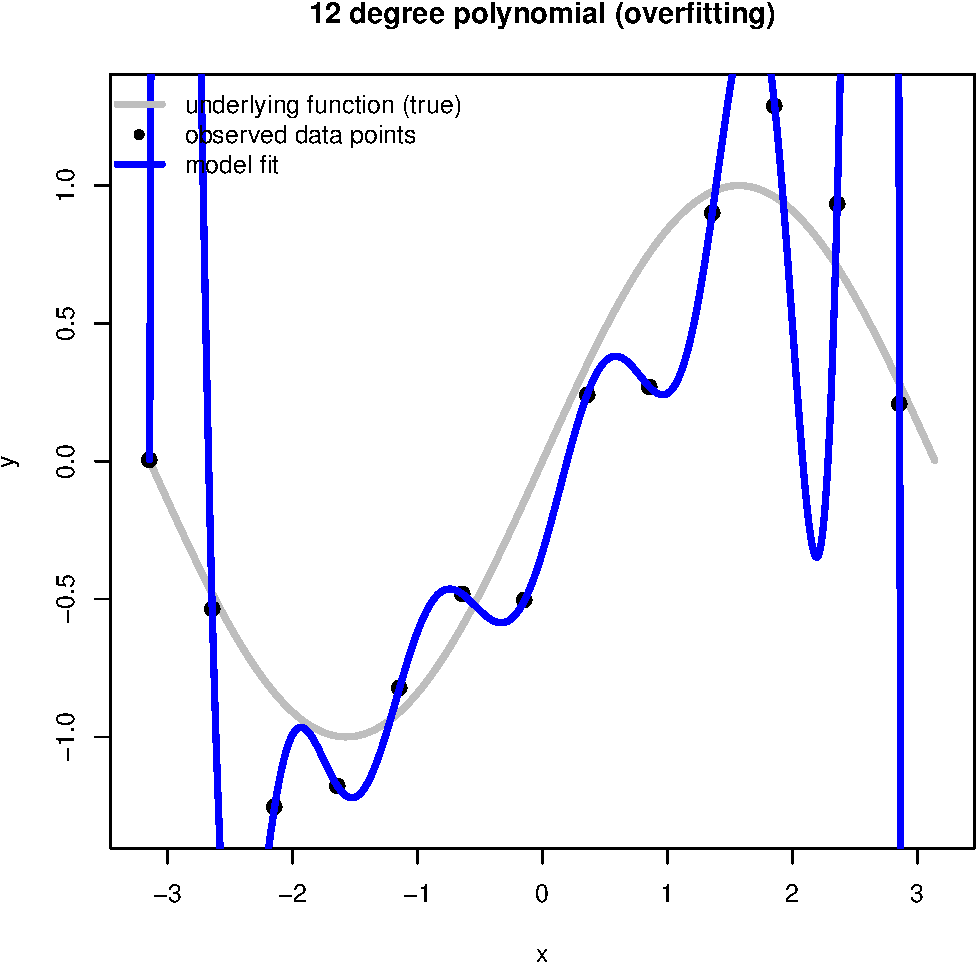
\includegraphics[width=0.333\textwidth]{polyFit12.pdf}
\end{center}
\end{frame}
%-------------------------------------------------------------------------------------------------%
\begin{frame}{Iris dataset}
\begin{center}
	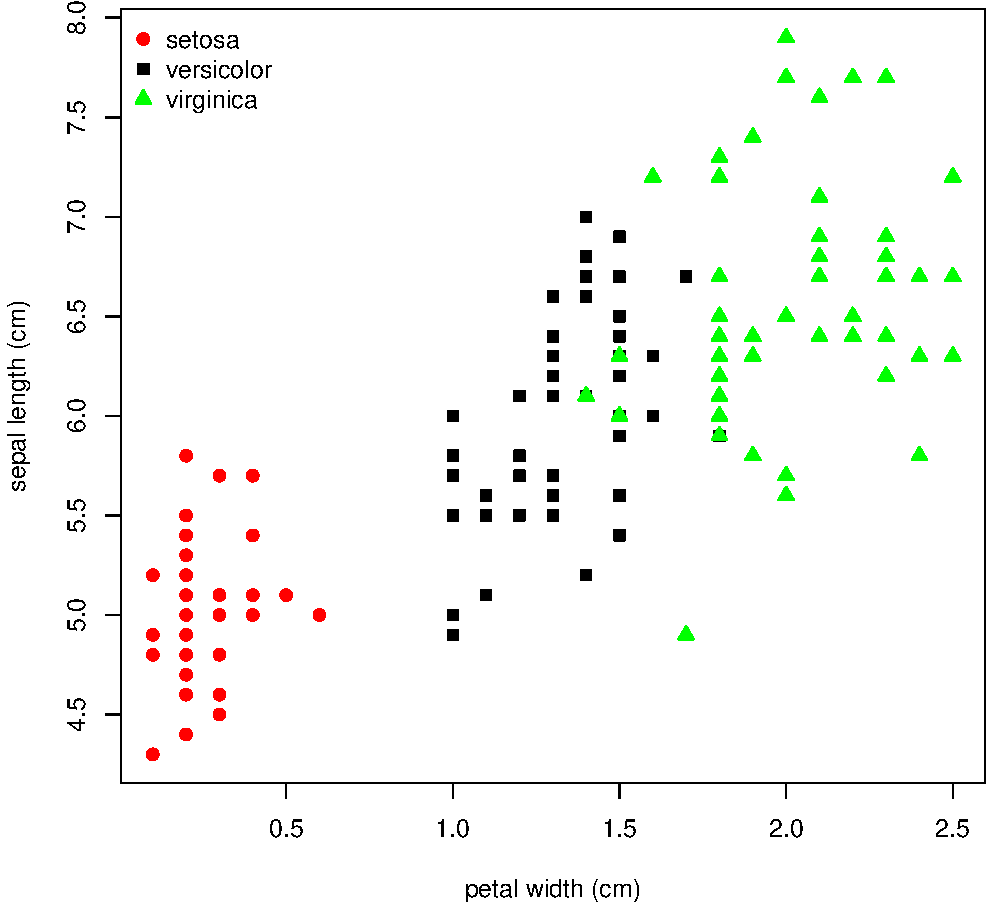
\includegraphics[width=0.74\textwidth]{irisPlot.pdf}
\end{center}
\end{frame}
%-------------------------------------------------------------------------------------------------%
\begin{frame}[fragile]
\frametitle{$k$-nearest neighbour ($k$NN)}
\begin{lstlisting}[style=RCode]
library(class)
fit <- knn(train, test, cl, k)
# train - training dataset (matrix or data frame)
# test - testing dataset (matrix or data frame)
# cl - corresponding label of the training dataset (factor)
# k - number of neighbours
\end{lstlisting}
\begin{enumerate}\addtolength{\itemsep}{0.5\baselineskip}
	\item<2-> Calculate distance between test point and every training data point 
	\item<3-> Find the $k$ training points closest to test point 
	\item<4-> Assign test point the majority vote of their class label
\end{enumerate}
%\vfill
%\textbf{Note}: $k$NN should \textit{only} be used with continuous predictors
\end{frame}
%-------------------------------------------------------------------------------------------------%
\begin{frame}{$k$-nearest neighbour}
	\begin{center}
		\includegraphics<1>[width=0.68\textwidth]{1nearestNeighbour.pdf}
		\includegraphics<2>[width=0.68\textwidth]{5nearestNeighbour.pdf}
		\includegraphics<3>[width=0.68\textwidth]{15nearestNeighbour.pdf}
		\includegraphics<4>[width=0.68\textwidth]{30nearestNeighbour.pdf}
	\end{center}
\end{frame}
%-------------------------------------------------------------------------------------------------%
\begin{frame}{$k$-nearest neighbour}
\begin{exampleblock}{Pros}
\begin{itemize}
	\item Simple and intuitive
	\item Works for multi-class problems
	\item Non-linear decision boundaries 
	\item $k$ easily tuned by cross-validation  
\end{itemize}
\end{exampleblock}
\vfill
\begin{alertblock}{Cons}
\begin{itemize}
	\item Can be computationally expensive as for every test point distance to every training data 
	points needs to be computed (the model is actually the whole training dataset) 
	\item Defining nearest by a distance metric can be ambiguous (for e.g when you have categorical predictors)
\end{itemize}
\end{alertblock}
\end{frame}
%-------------------------------------------------------------------------------------------------%
\begin{frame}[fragile]
\frametitle{Decision trees}
\begin{lstlisting}[style=RCode]
library(tree)
fit <- tree(formula, data)
# OR
library(rpart)
fit <- rpart(formula, data)
# formula - an R formula expression e.g y ~ x1+x2
# data - data frame
\end{lstlisting}
\begin{enumerate}\addtolength{\itemsep}{0.5\baselineskip}
	\item<2-> Divide data into left-right (yes-no) by an axis parallel split using \textit{one} predictor 
	\item<3-> The best split is found by maximising information gain/lowering entropy
	\item<4-> Repeat 1 to 2 until all data is correctly classified or some stopping rule reached
\end{enumerate}
\end{frame}
%-------------------------------------------------------------------------------------------------%
\begin{frame}{Decision trees - The Model}
\begin{center}
	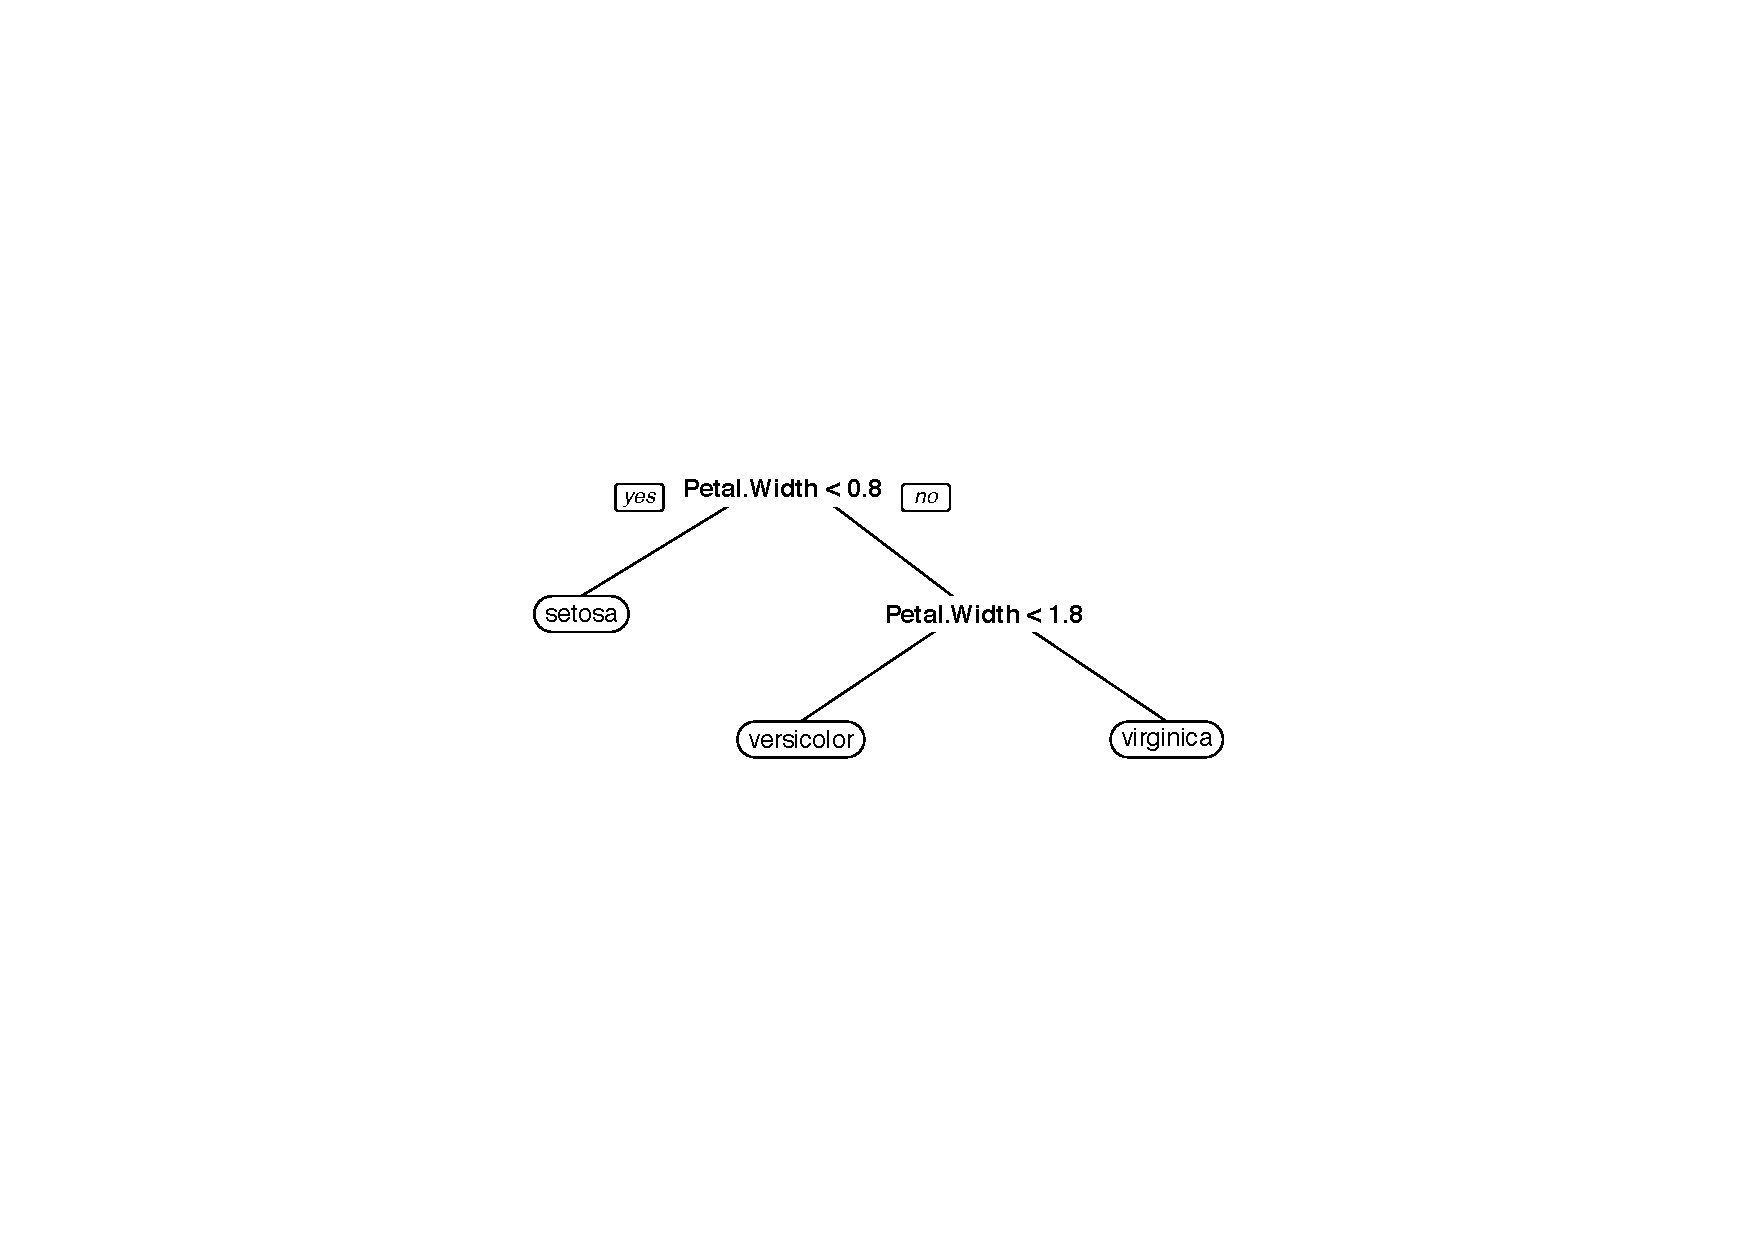
\includegraphics[width=\textwidth]{crudeTree.pdf}
\end{center}
\end{frame}
%-------------------------------------------------------------------------------------------------%
\begin{frame}{Decision trees - The Model}
\begin{center}
	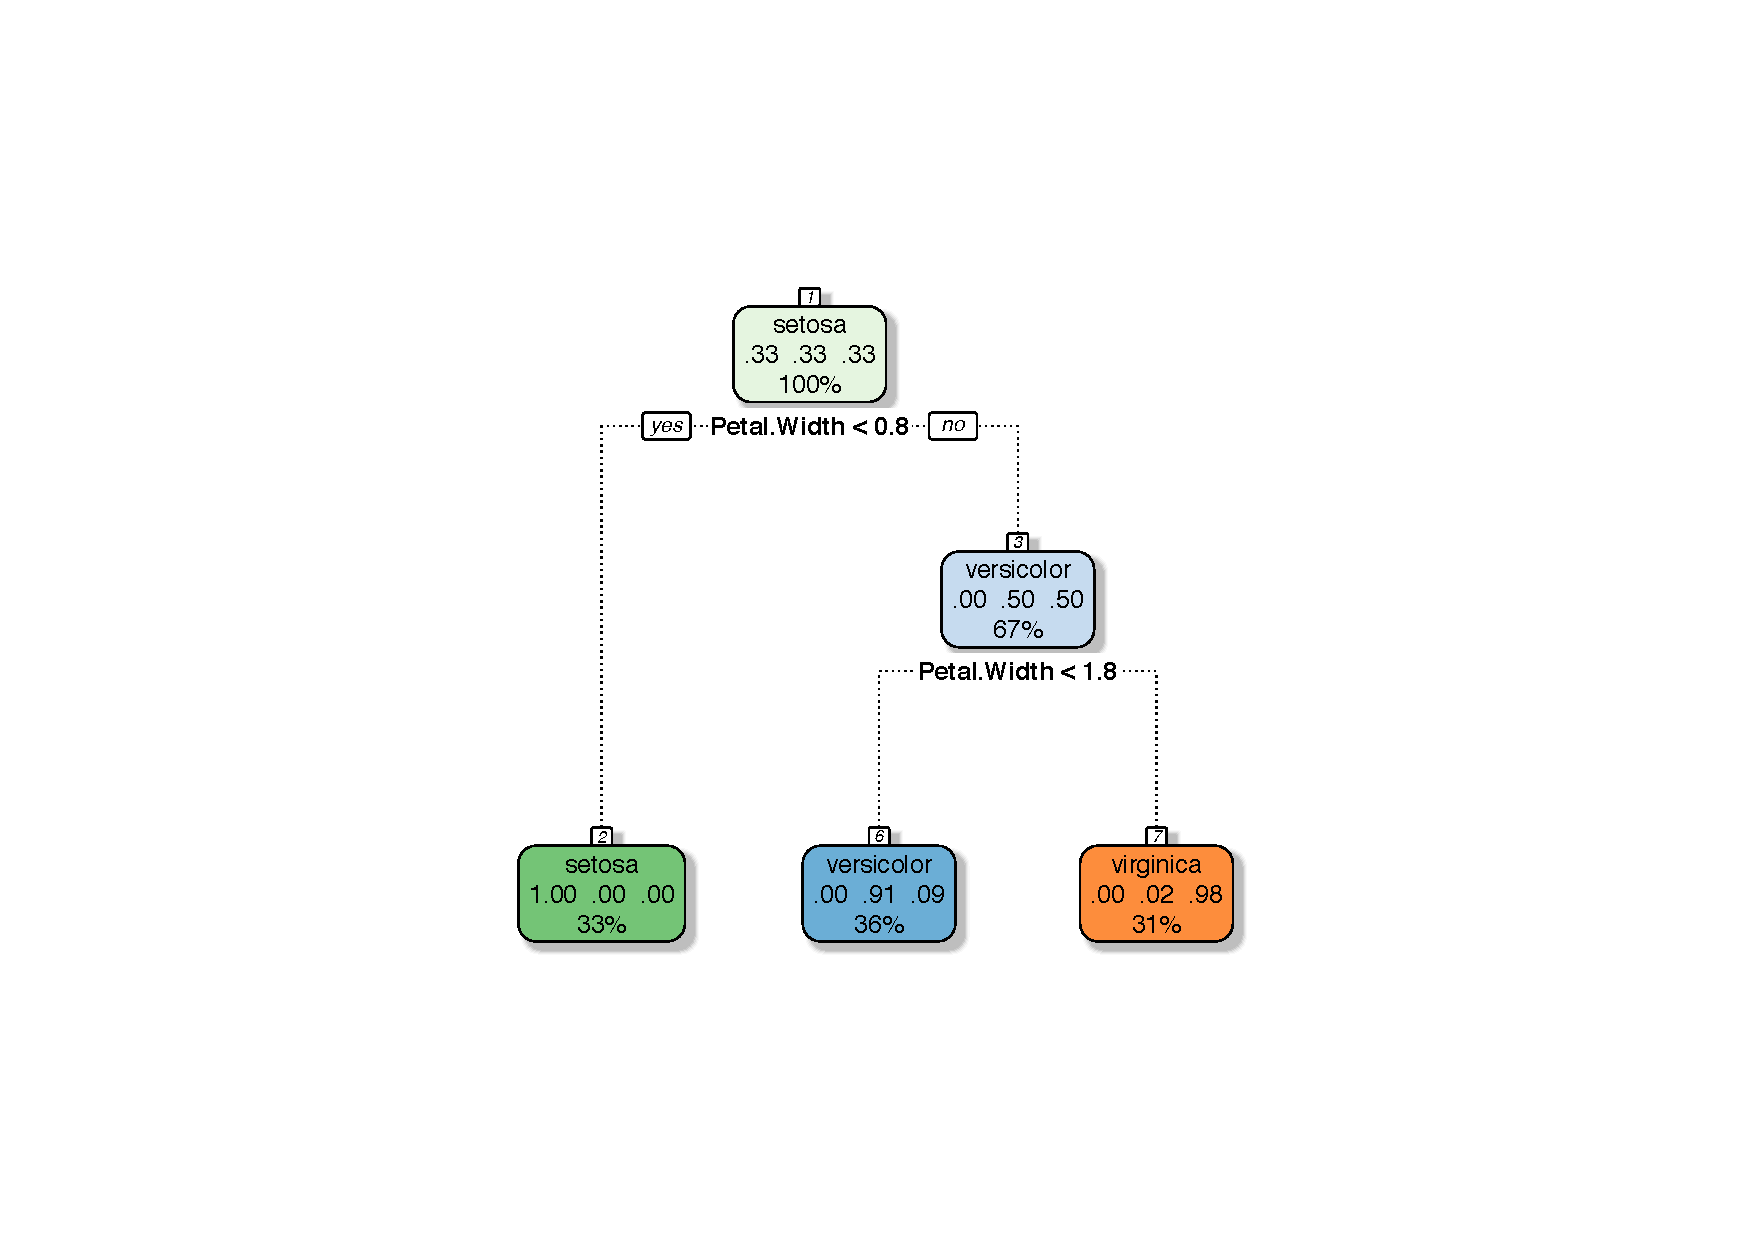
\includegraphics[width=0.7\textwidth]{niceTree.pdf}	
\end{center}
\end{frame}
%-------------------------------------------------------------------------------------------------%
\begin{frame}{Decision boundaries}
\begin{center}
	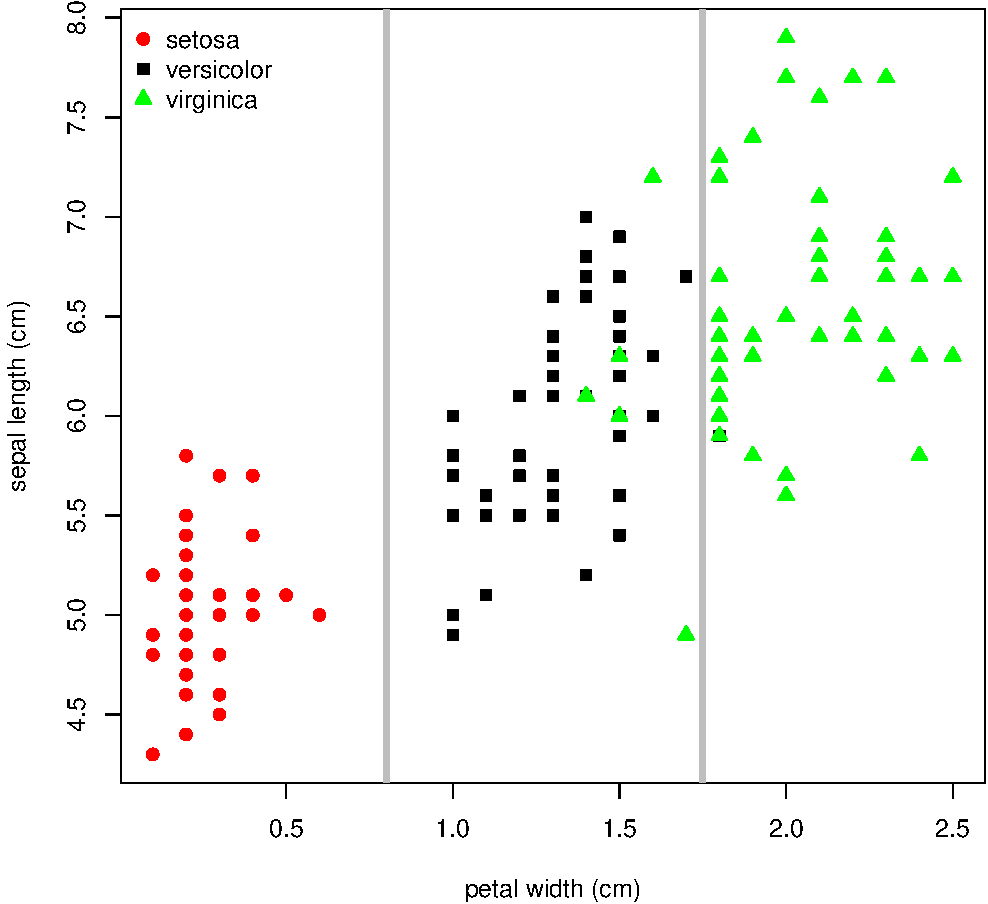
\includegraphics[width=0.74\textwidth]{irisPlotBound.pdf}
\end{center}
\end{frame}
%-------------------------------------------------------------------------------------------------%
\begin{frame}{Decision trees}
\begin{exampleblock}{Pros}
\begin{itemize}
	\item Model is very interpretable and can be directly used to generate rules
	\item Computationaly inexpensive to train and evaluate 
	\item Handle both categorical and continuous data
	\item Robust to outliers
\end{itemize}
\end{exampleblock}
\vfill
\begin{alertblock}{Cons}
\begin{itemize}
	\item Can easily overfit the data
	\item Predictive accuracy can be poor
	\item Small changes to training data may lead to a completely different tree
\end{itemize}
\end{alertblock}
\end{frame}
%-------------------------------------------------------------------------------------------------%
\begin{frame}{Random forests}
\begin{itemize}\addtolength{\itemsep}{0.1\baselineskip}
	\item Decision trees are intuitive but suffer from overfitting which significantly affect their predictive accuracy
	\item \textit{Pruning}, to ``trim'' the tree back, help reduce this overfit
	\item \textit{Ensemble} methods such as Random Forests are a better alternative
	\item \textbf{Rationale}: Instead of one tree, grow a \textit{forest}, where every bushy tree (no pruning) is a bit different,
	then average predictions over all trees
\end{itemize}
\vfill
\begin{center}
	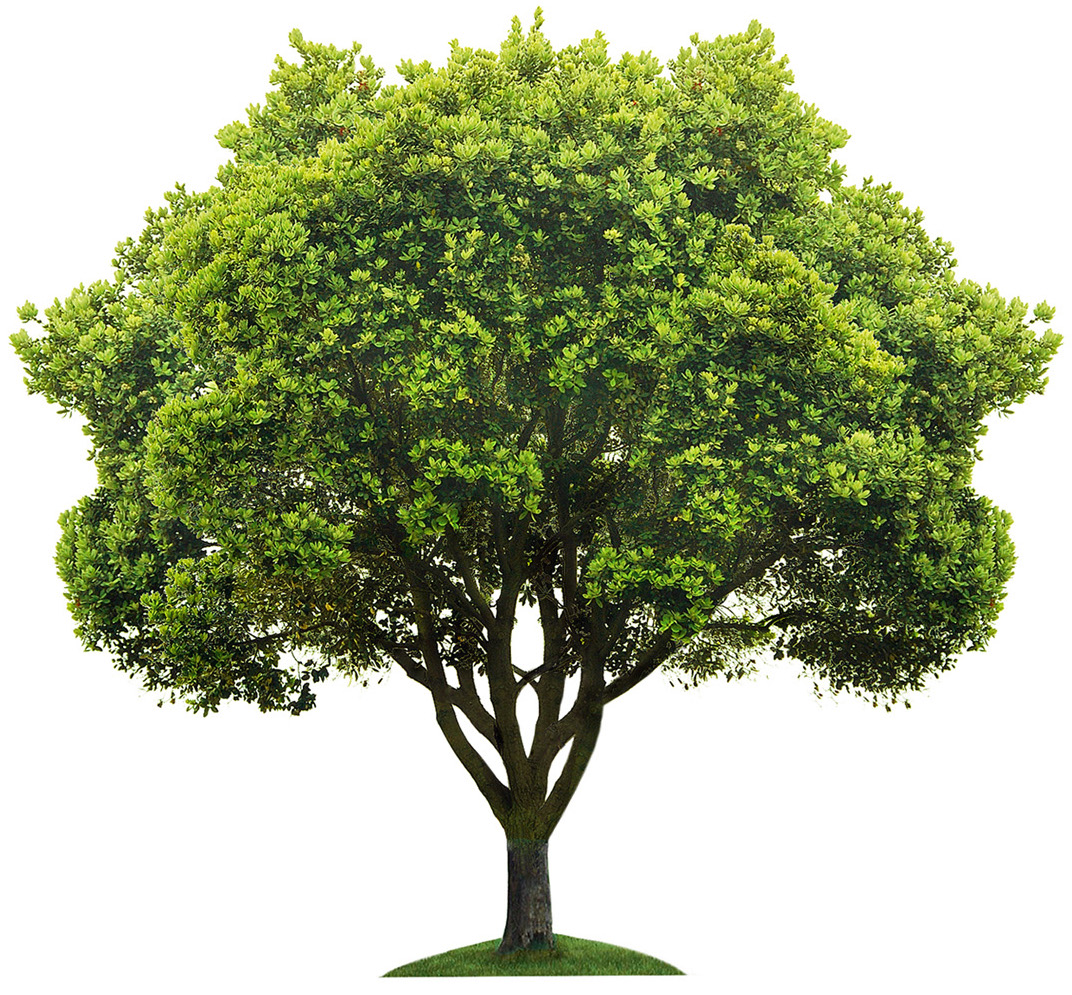
\includegraphics[width=0.32\textwidth]{tree.jpg}
	\Huge $\Rightarrow$ \normalsize
	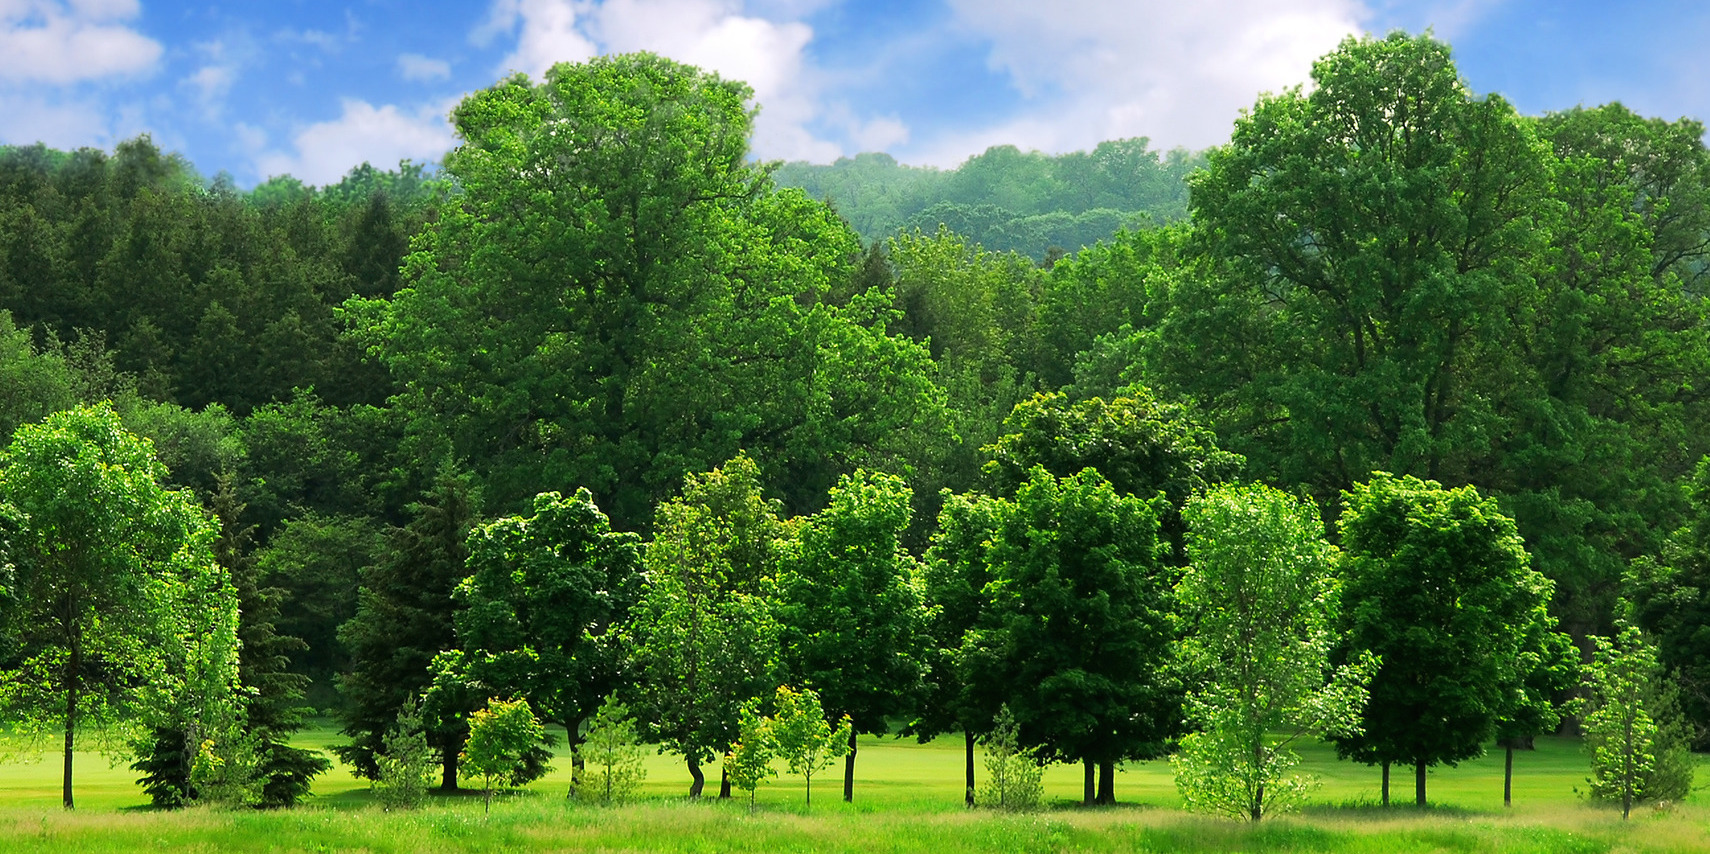
\includegraphics[width=0.58\textwidth]{forest.jpg}
\end{center}
\end{frame}
%-------------------------------------------------------------------------------------------------%
\begin{frame}[fragile]
\frametitle{Random forests}
\begin{lstlisting}[style=RCode]
library(randomForest)
fit <- randomForest(formula, data, ntree, mtry)
# formula - an R formula expression e.g y ~ x1+x2
# data - data frame
# ntree - number of trees in forest
# mtry - number of predictors randomly sampled as candidates at each split (default is sqrt(num of covariates))
\end{lstlisting}
\begin{enumerate}\addtolength{\itemsep}{0.5\baselineskip}
	\item<2-> Grow $ntree$ bushy trees (no pruning) which are de-correlated from each other
	\item<3-> Forest randomness is induced by:
		\begin{itemize}
			\item<3-> Bagging (\textbf{B}ootstrap \textbf{AGG}regat\textbf{ING}), each tree is trained
			on a subset of the data randomly sampled with replacement
			\item<3-> For every tree split consider only $mtry$ predictors as candidates for that split 
		\end{itemize}
	\item<4-> Average predictions from all $ntree$ trees
\end{enumerate}
\end{frame}
%-------------------------------------------------------------------------------------------------%
\begin{frame}{De-correlated bushy trees in the forest}
	\begin{center}
		\includegraphics<1>[width=0.68\textwidth]{treeFit1.pdf}
		\includegraphics<2>[width=0.68\textwidth]{treeFit2.pdf}
	\end{center}
\end{frame}
%-------------------------------------------------------------------------------------------------%
\begin{frame}{Variable importance}
	\begin{center}
		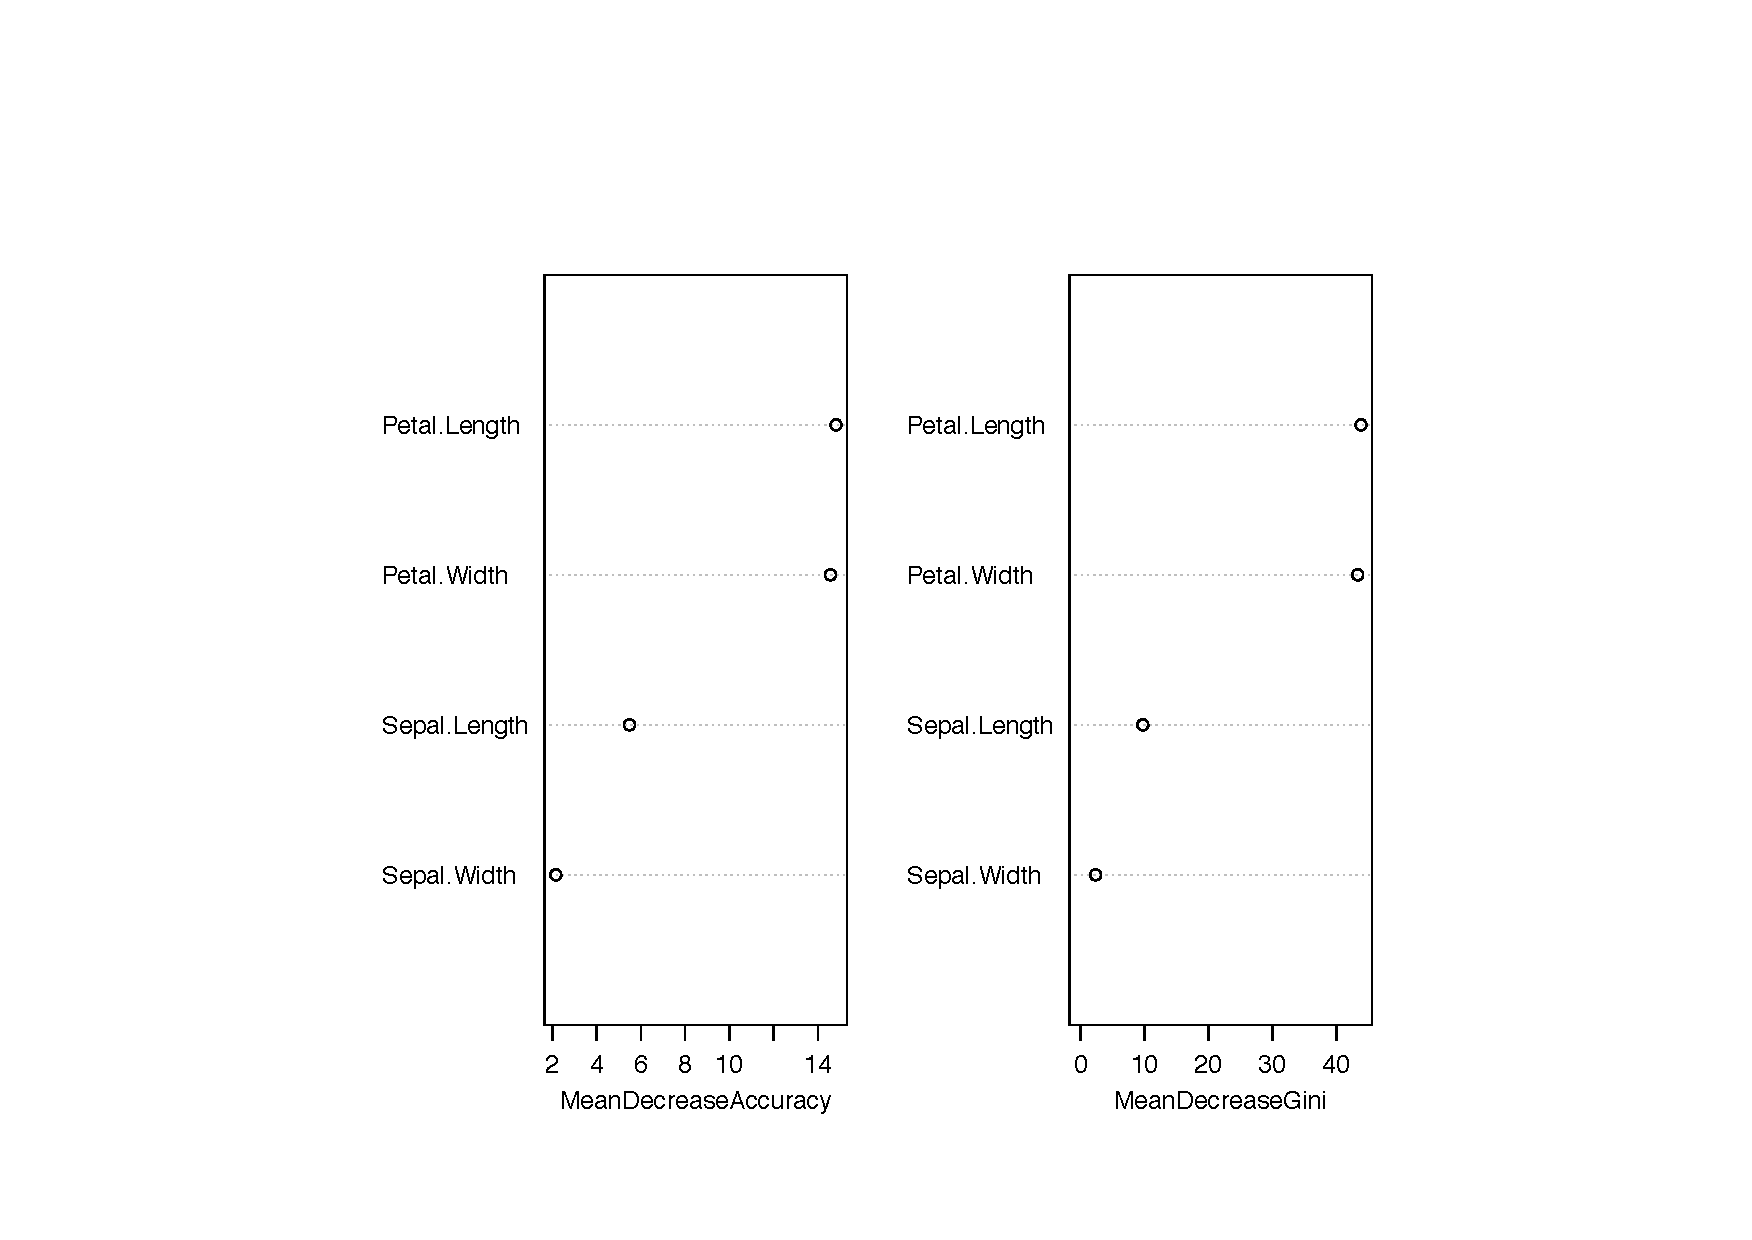
\includegraphics[width=0.8\textwidth]{varImportance.pdf}
	\end{center}
\end{frame}
%-------------------------------------------------------------------------------------------------%
\begin{frame}{Random forests}
\begin{exampleblock}{Pros}
\begin{itemize}
	\item State-of-the-art predictive accuracy
	\item Can handle thousands of both categorical and continuous predictors without variable deletion
	\item Robust to outliers
	\item Estimates the importance of every predictor
	\item Out-of-bag error (unbiased estimate of test error for every tree built)
	\item Can cope with unbalanced datasets by setting class weights
\end{itemize}
\end{exampleblock}
\vfill
\begin{alertblock}{Cons}
\begin{itemize}
	\item Harder to interpret then plain decision trees
\end{itemize}
\end{alertblock}
\end{frame}
%-------------------------------------------------------------------------------------------------%
\begin{frame}{Support vector machines (SVM)}
Which is the best separating line?
	\begin{center}
		\includegraphics<1>[width=0.7\textwidth]{svmSepLine1.pdf}
		\includegraphics<2>[width=0.7\textwidth]{svmSepLine2.pdf}
		\includegraphics<3>[width=0.7\textwidth]{svmSepLine3.pdf}
		\includegraphics<4>[width=0.7\textwidth]{svmSepLine4.pdf}
	\end{center}
\end{frame}
%-------------------------------------------------------------------------------------------------%
\begin{frame}{Support vector machines}
\textbf{Rationale}: Maximise the \textit{margin}, the distance to separating hyperplane
\begin{center}
		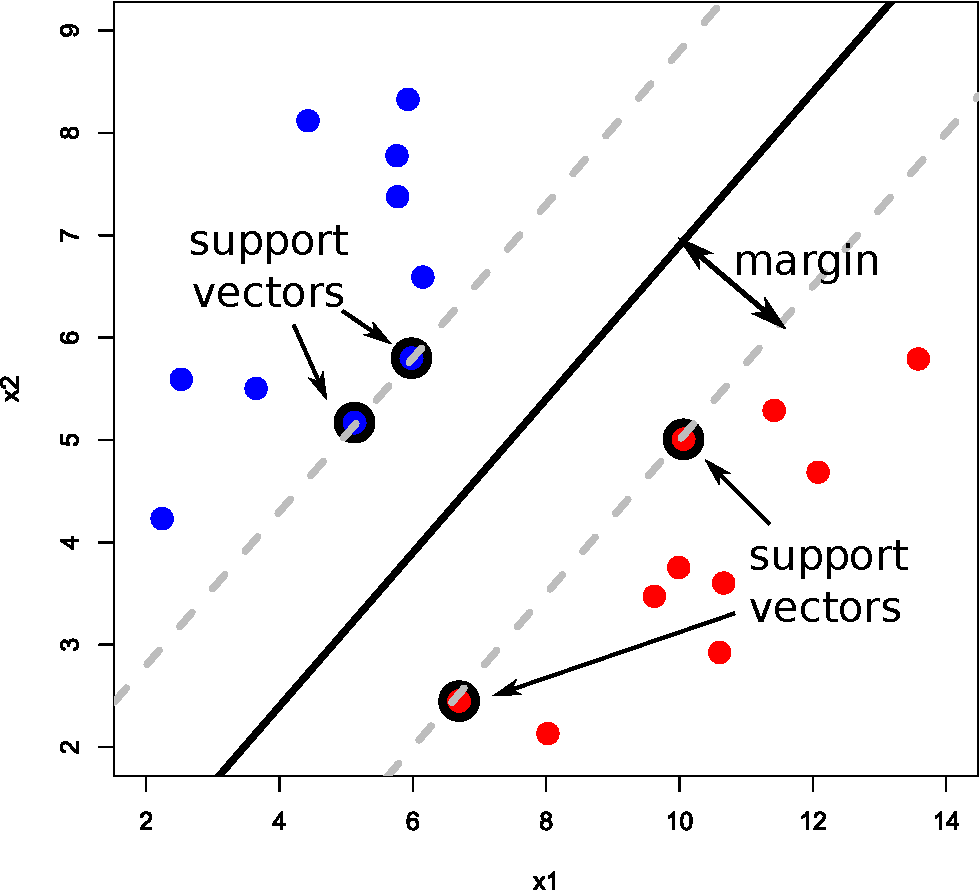
\includegraphics[width=0.7\textwidth]{svmSketch.pdf}
\end{center}
\end{frame}
%-------------------------------------------------------------------------------------------------%
\begin{frame}{Support vector machines}
If it's something weird and it don't look good. Who ya gonna call?\\
Ghostbusters?\\ 
\textit{Close}, we need alternate dimensions to make them linearly separable
\vfill
\begin{center}
		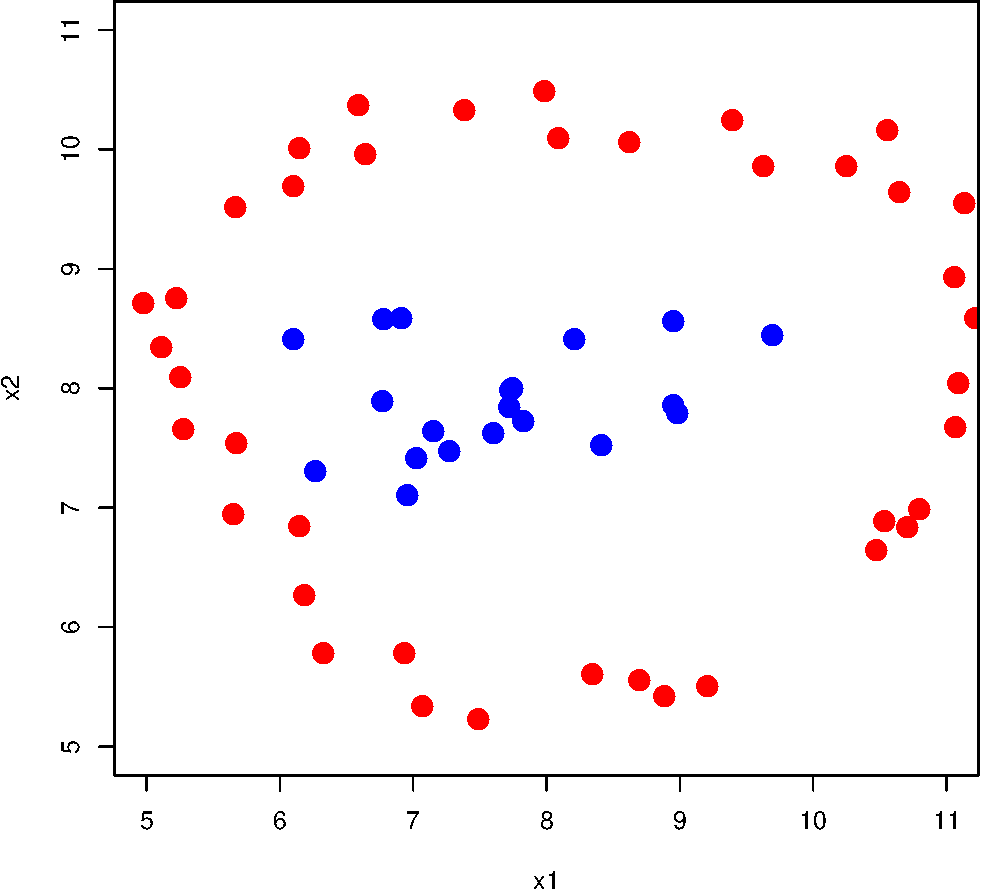
\includegraphics[width=0.6\textwidth]{svmNonLinear1.pdf}
\end{center}
\end{frame}
%-------------------------------------------------------------------------------------------------%
\begin{frame}{Support vector machines}
\begin{itemize}
	\item Map data to a higher dimensional space where classes are linearly separable
	(artificially increasing number of predictors)
	\item $(x_1,\ x_2) \rightarrow (1,\ x_1,\ x_2,\ x_1x_2,\ x_1^2,\ x_2^2)$
	\item Hyperplane in \textit{new} space is a conic section in \textit{original} space 
\end{itemize}
\begin{center}
		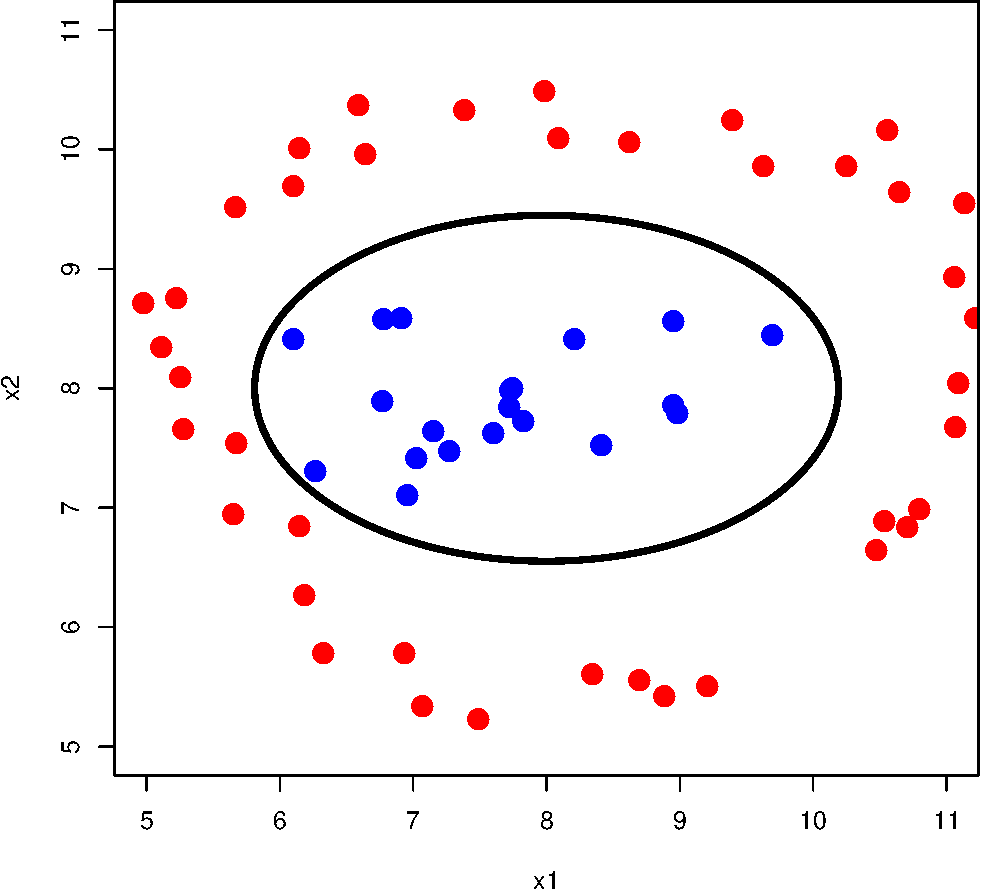
\includegraphics[width=0.55\textwidth]{svmNonLinear2.pdf}
\end{center}
\end{frame}
%-------------------------------------------------------------------------------------------------%
\begin{frame}{Support vector machines: Simple example from 1D to 2D}
\begin{center}
		\visible<1->{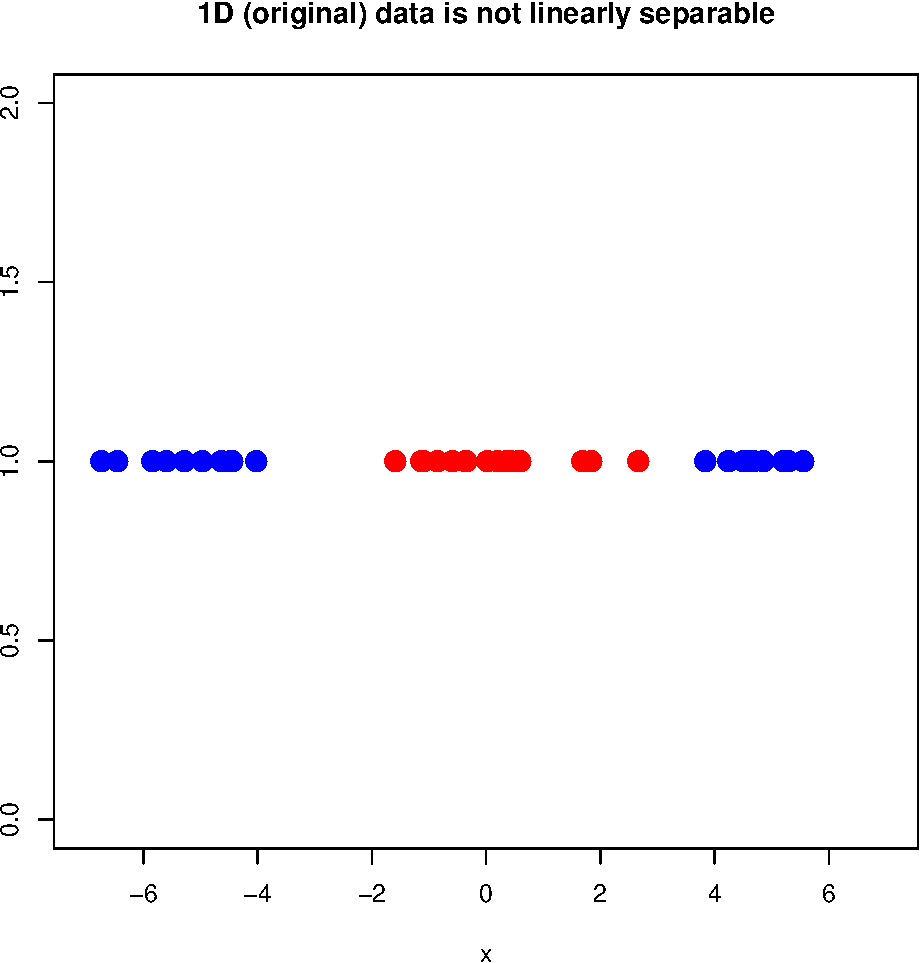
\includegraphics[width=0.47\textwidth]{svmSimple1.pdf}}
		\visible<2->{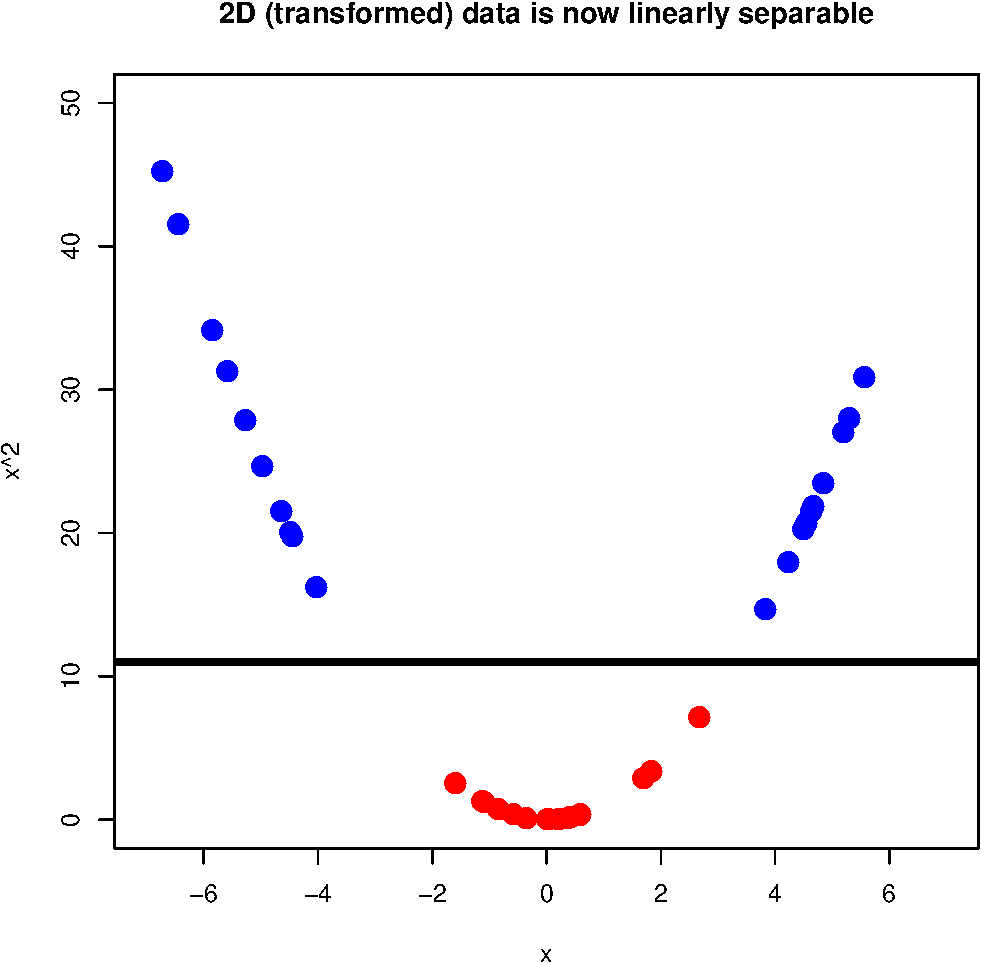
\includegraphics[width=0.50\textwidth]{svmSimple2.pdf}}
\end{center}
\end{frame}
%-------------------------------------------------------------------------------------------------%
\begin{frame}{Support vector machines - The kernel trick}
\begin{itemize}\addtolength{\itemsep}{0.5\baselineskip}
	\item So our solution is to blow up the dimensions?
	\item But what about the ``curse of dimensionality''?
	\item Very computationally expensive to work in high dimensions
\end{itemize}
\vfill
\visible<2->{\begin{framed}
\textbf{Kernel trick} to the rescue! We work in an \textit{implict} feature space, that is, data is 
never explicitly computed in higher dimensions. Instead we only need to compute the pair-wise inner product.  
\end{framed}
\vfill
\textbf{p.s} Kernel methods are mathematically intricate and beyond the scope of this workshop so I will stop here}
\end{frame}
%-------------------------------------------------------------------------------------------------%
\begin{frame}[fragile]
\frametitle{Support vector machines}
\begin{lstlisting}[style=RCode]
library(e1071)
fit <- svm(formula, data, type, kernel)
# formula - an R formula expression e.g y ~ x1+x2
# data - data frame
# type - whether the problem is classification or regression
# kernel - the kernel function e.g "linear" or "radial basis"
\end{lstlisting}
\begin{enumerate}\addtolength{\itemsep}{0.5\baselineskip}
	\item Choose carefully a kernel function
	\item Run optimiser to find maximum margin
\end{enumerate}
\end{frame}
%-------------------------------------------------------------------------------------------------%
\begin{frame}{Support vector machines}
\begin{center}
		\includegraphics<1>[width=0.68\textwidth]{svmLinear.pdf}
		\includegraphics<2>[width=0.68\textwidth]{svmRBF.pdf}
\end{center}
\end{frame}
%-------------------------------------------------------------------------------------------------%
\begin{frame}{Support vector machines}
\begin{exampleblock}{Pros}
\begin{itemize}
	\item State-of-the-art predictive accuracy
	\item Less prone to overfitting
	\item Only need to store the support vectors for the predictive model
	\item Picking the right kernel gives you flexibility and predictive power
	\item Global optimum guaranteed
\end{itemize}
\end{exampleblock}
\vfill
\begin{alertblock}{Cons}
\begin{itemize}
	\item Unintuitive/a black box
	\item Cannot visualise the feature space
\end{itemize}
\end{alertblock}
\end{frame}
%-------------------------------------------------------------------------------------------------%
\end{document}
%-------------------------------------------------------------------------------------------------%
% End of Document
%-------------------------------------------------------------------------------------------------%